\chapter{Evaluation}
\label{sec:evaluation} 

\section{Evaluation Procedure}
The developed system was evaluated with four modeling experts to assess its usability and perceived usefulness, as well as to gather feedback on potential improvements and additional features.

Each evaluation session followed a semi-structured procedure and lasted approximately 40 minutes. It began with a brief demonstration of the system's workflow and main features. After that, the participants were asked to complete two tasks. The first was an exploratory task based on a synthetic B2B order processing scenario consisting of two wiki-style documents in DOCX format (see Appendix~\ref{app:order}). It was designed to help participants familiarize themselves with the system. The second was a more realistic process modeling task based on an open-source SOP document \footnote{\href{https://dnrc.mt.gov/_docs/forestry/Wildfire/agreements-plans-guides/DNRC-Manuals/300-Fire-Business-Manual/Appendix-300-Manual/2023_Fire_Contract_PMT_SOP.pdf}{DNRC SOP Document}} in PDF format. For both tasks, participants were not given strict instructions on how to proceed, allowing them to explore the system freely. If time permitted, participants could additionally use the system with their own documents. 

Following task completion, participants completed a questionnaire including the following questions: \\
(1) What aspects of the tool did you like while using it? \\
(2) What aspects of the tool did you not like or find problematic? \\
(3) What improvements or additional features would you most like to see in the tool? \\
(4) If you needed to model processes from documents in the future, would you consider using this tool? Why or why not?

\section{Evaluation Results}
\subsection{Overall Perception}
Overall, participants perceived the tool as usable and intuitive, and capable of supporting document-based process modeling tasks within a unified environment. The Figure (See Figure~\ref{fig:eva_expert2_task1}). Figure~\ref{fig:modeling-result-task2} shows the modeling results from one expert for the first and second tasks, respectively. 

The feedback to each functionality is summarized within the table~\ref{table:evaluation-results}. Due to different background of the expert, the perspectives varied. Details of the feedback are described in the following sections.
\begin{figure}[H]
    \centering
    \caption{Modeling result} 
    \floatfoot{Modeling result of an expert for the first task.}
    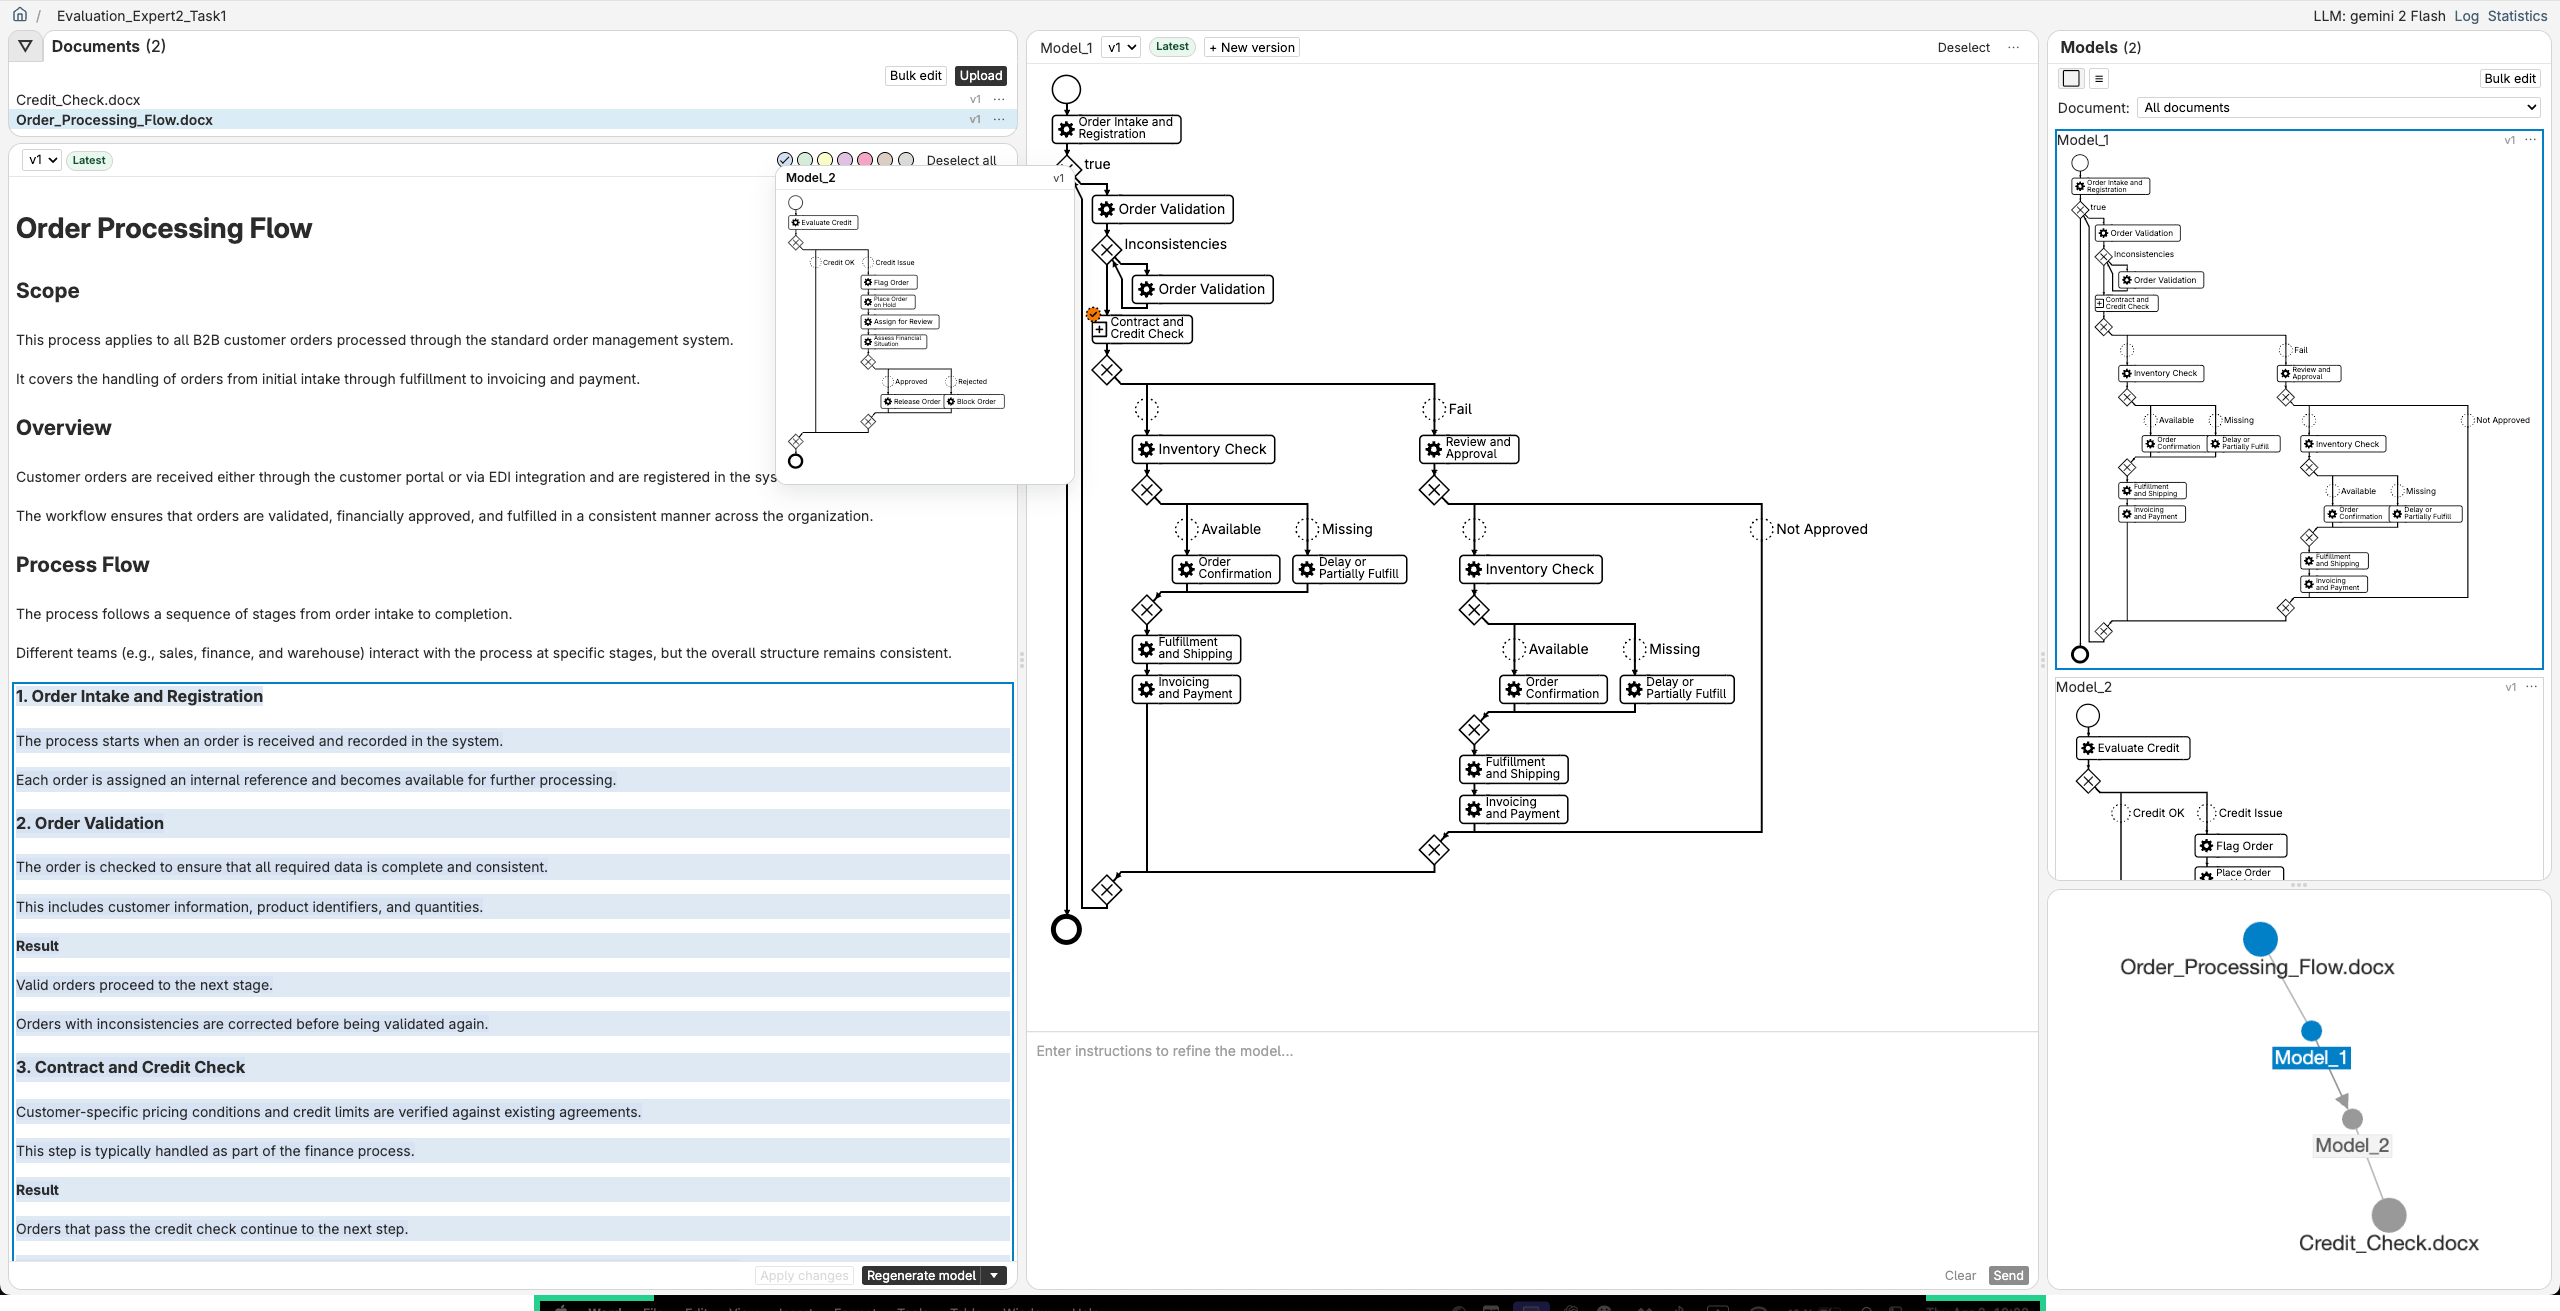
\includegraphics[width=1\textwidth]{images/eva_expert2_task1.png}
    \label{fig:eva_expert2_task1}
\end{figure}

\begin{figure}[H]
    \centering
    \caption{Modeling result}
\floatfoot{Modeling result of an expert for the second task.}
    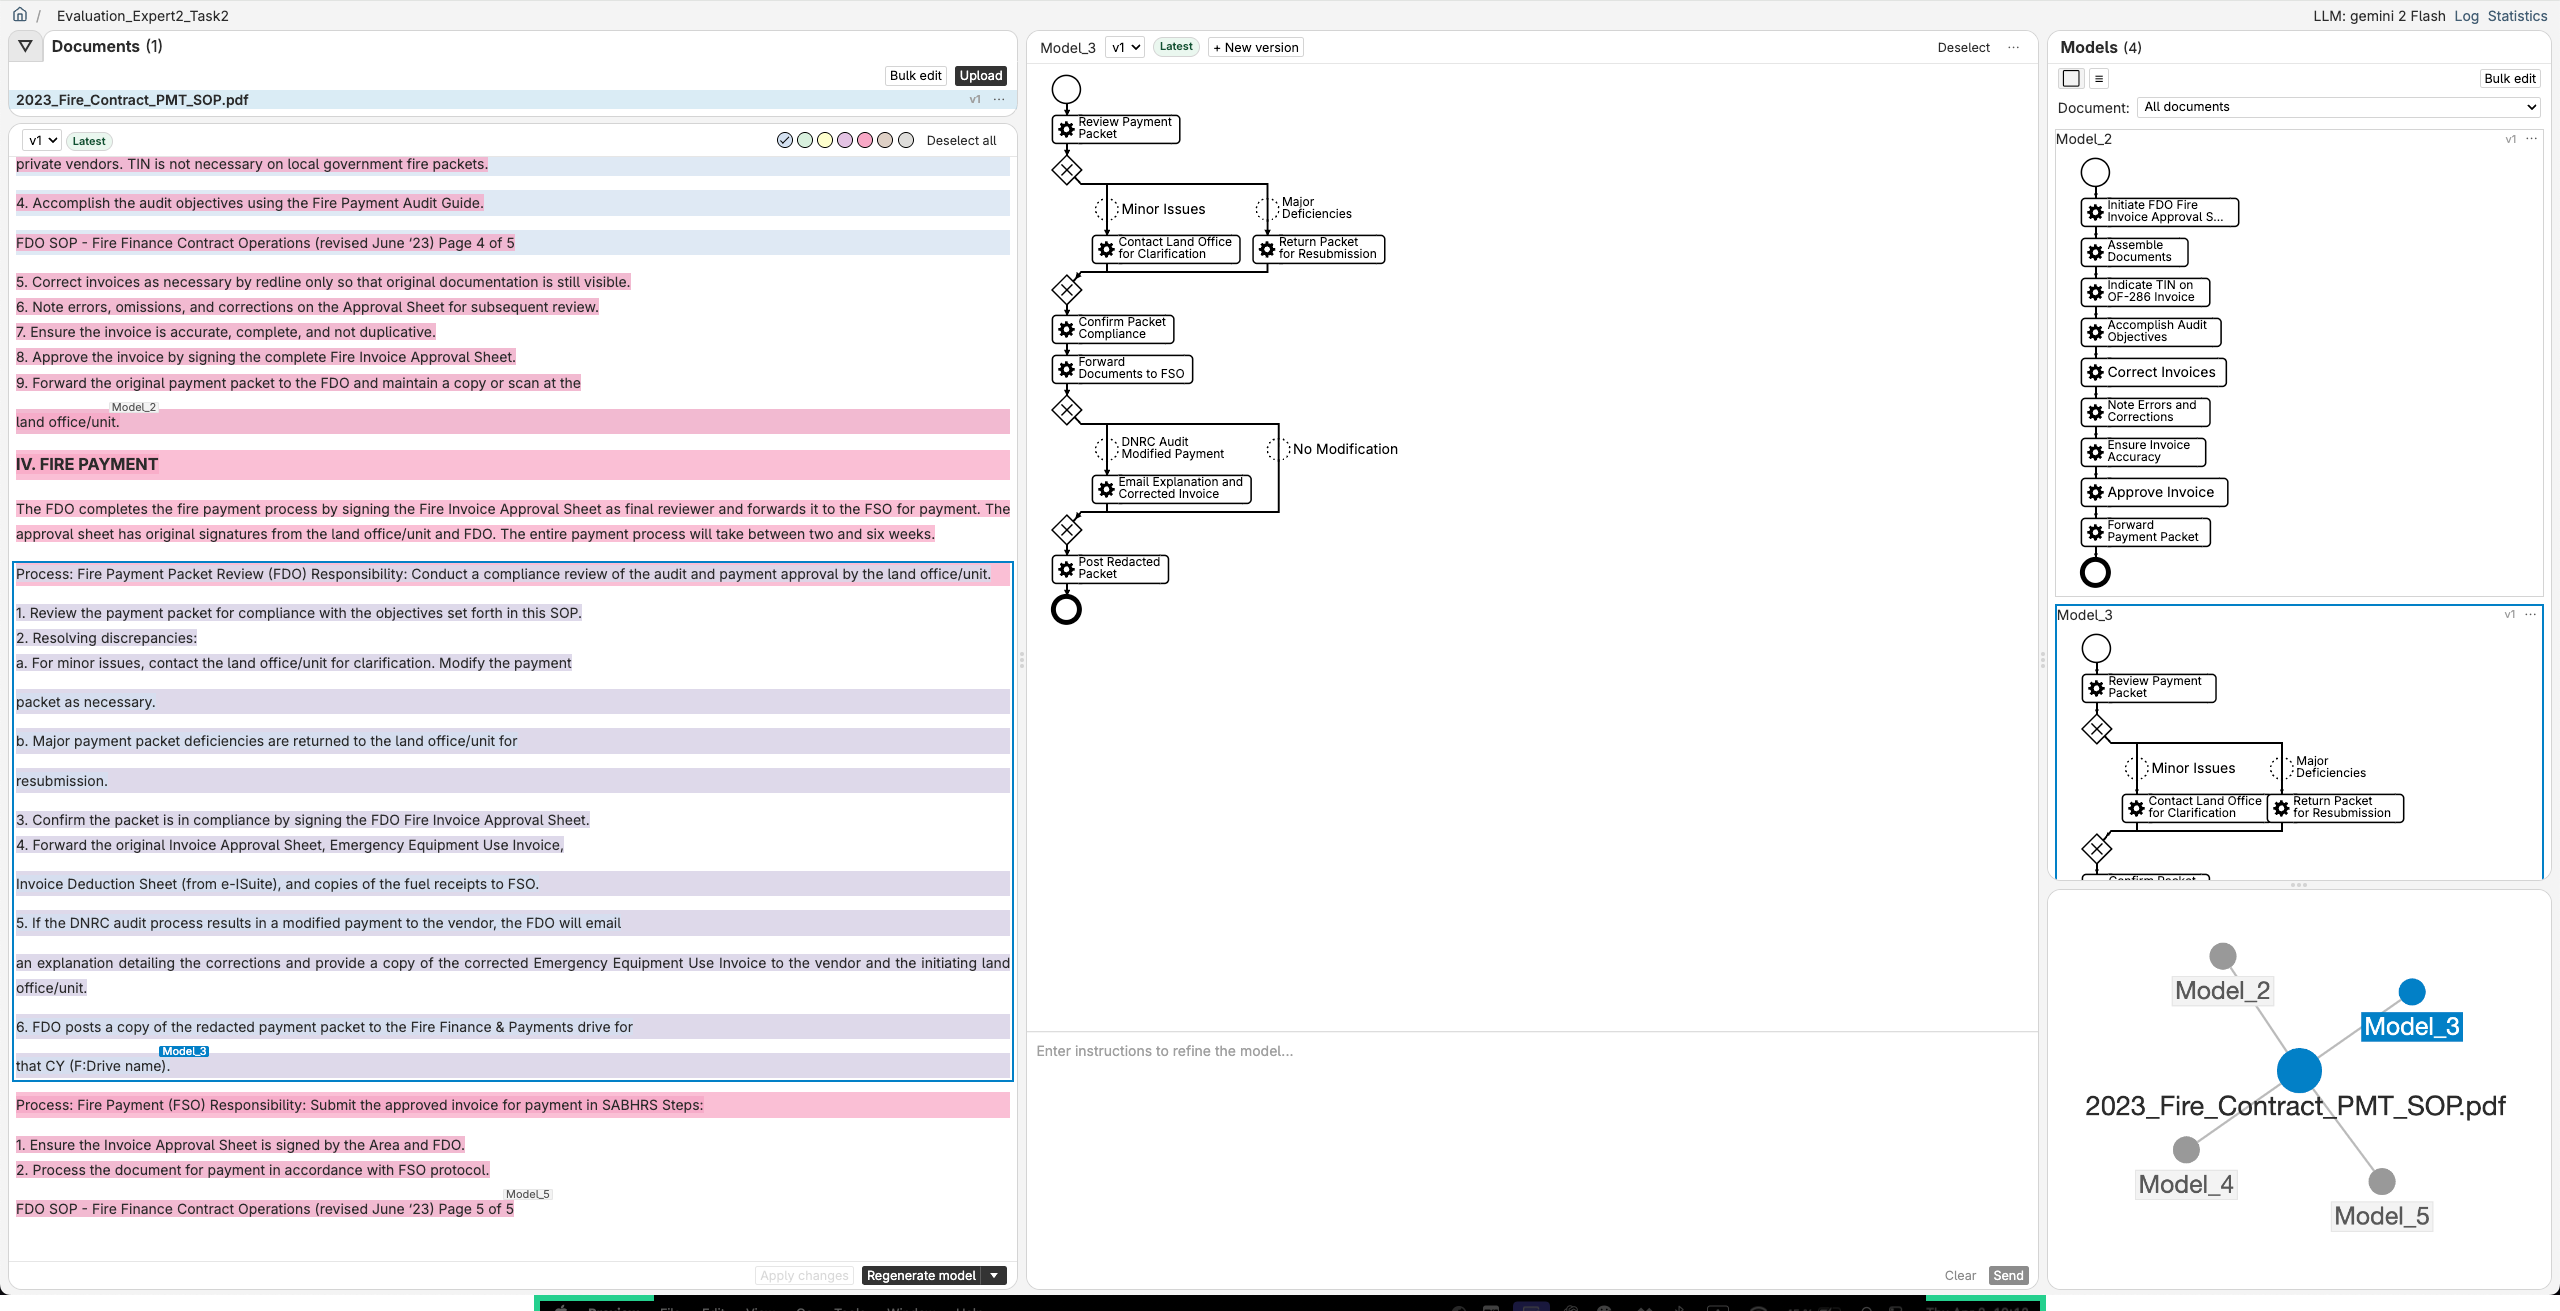
\includegraphics[width=1\textwidth]{images/eva_expert2_task2.png}
    \label{fig:modeling-result-task2}
\end{figure}


\begin{table}[H]
\centering
\caption{Summary of Evaluation Results by Functionality}
 \floatfoot{n = number of participants who mentioned each item}
\label{table:evaluation-results}
\begin{tabular}{p{3cm} p{4cm} c p{4.5cm} c}
\toprule
\textbf{Functionality} & \multicolumn{2}{c}{\textbf{Positive Aspects}} & \multicolumn{2}{c}{\textbf{Challenges and Limitations}} \\
\cmidrule(lr){2-3} \cmidrule(lr){4-5}
 & \textbf{Item} & \textbf{n} & \textbf{Item} & \textbf{n} \\
\midrule
Document Interaction &  &  & Readability issue & 1 \\
\midrule
\multirow{2}{3cm}{Integrated LLM-based Process Modeling }
& Fast & 2 & Unnecessary review step of the first generated model & 2 \\ 
\cmidrule(lr){2-3} \cmidrule(lr){4-5}
& Good quality & 2 & Lack of transparency in regeneration logic & 1\\
\midrule
Augmented Model Data
& Well-considered & 2 &  &  \\
\midrule
Traceability
& Clear & 1 & Lack of fine-grained link between actual used text and model & 2 \\
\midrule
Process-Subprocess Relationship
& Convenient & 3 &  &  \\
\midrule
Model Versioning
& Helpful & 3 &  &  \\
\midrule
Project Graph
& Helpful for larger systems & 1 & Node types not clear & 1 \\
\midrule
Log and Statistics
& Potentially useful for analysis & 1 &  &  \\
\bottomrule
\end{tabular}


\end{table}



\subsection{Positive Aspects}

\subsection{Challenges in Interaction and Use}
 
\subsection{Potential Improvements and Additional Features}

\section{Additional Observations}

Besides the gathered feedback, some findings regarding user behaviour and interaction are observed during the evaluation.

While most participants tended to select larger portions of text when starting with a new document, some preferred to begin with building models for smaller segments. These different strategies are illustrated in Figure~\ref{fig:text-selection-strategies}.
\begin{figure}[H]
    \centering
    \caption{Different modeling strategies}
    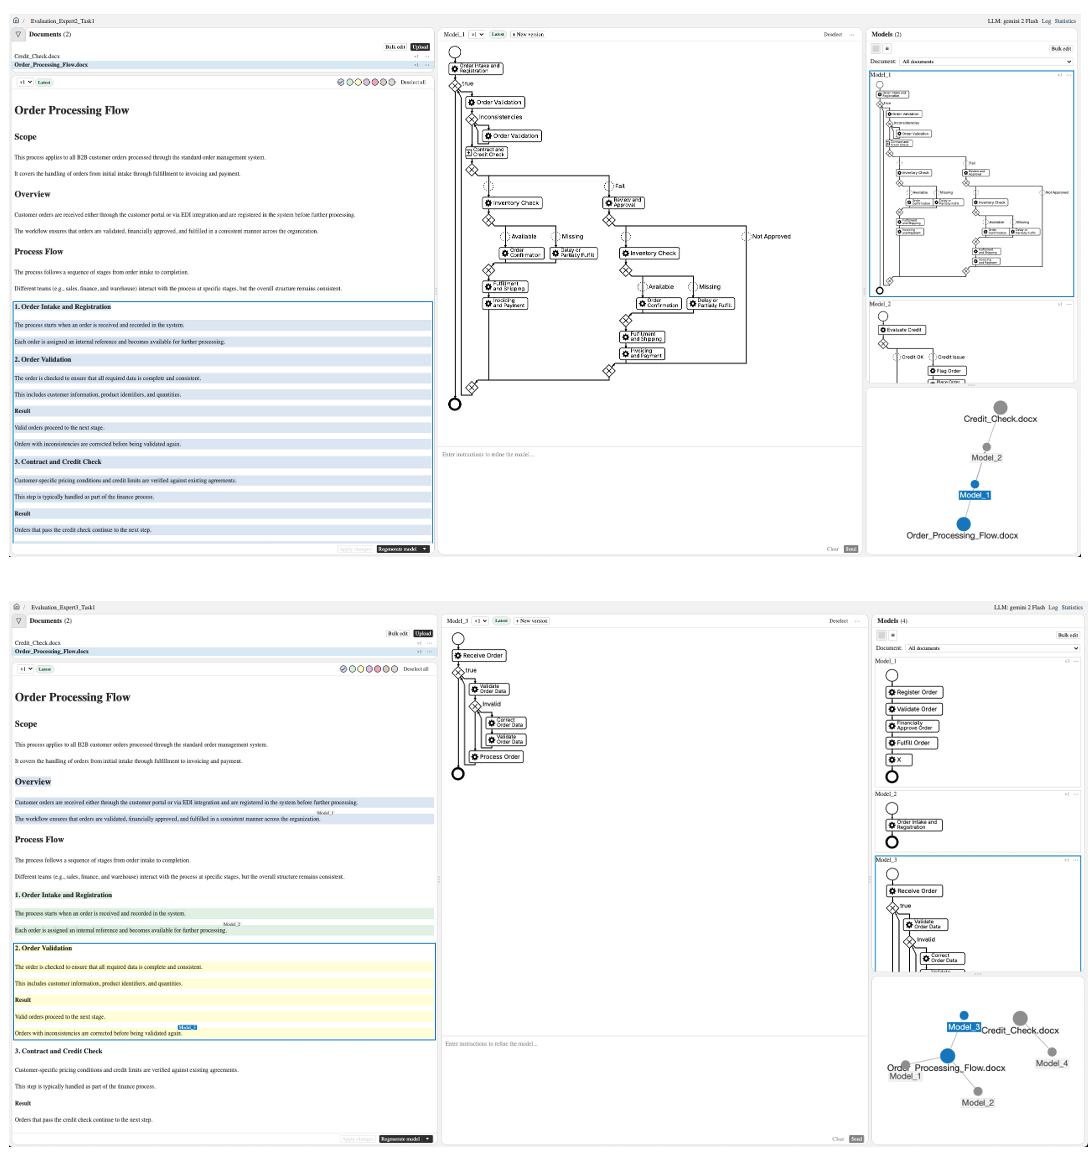
\includegraphics[width=0.7\textwidth]{images/Screenshot1.png}
    \floatfoot{Different modeling strategies observed during task execution (above: larger part selection; below: step-by-step selection)}
    \label{fig:text-selection-strategies}
\end{figure}


